\documentclass[12pt]{article}

\usepackage{fullpage}
\usepackage{fancybox} 
\usepackage{amssymb}
\usepackage{charter}
\usepackage{verbatim}
\usepackage{graphicx}
\usepackage[margin=1in]{geometry}
\usepackage{tikz}
\usepackage{mathtools}
\setlength{\textwidth}{7in}
\setlength{\evensidemargin}{-0.24in}
\setlength{\oddsidemargin}{-0.24in}
\setlength{\textheight}{9.45in}
\setlength{\topmargin}{-0.45in}
\setlength{\parindent}{0.3in}
\headheight12pt
\headsep16pt
\pagestyle{myheadings}
\newcounter{ques}
\newenvironment{question}{\stepcounter{ques}{\noindent\bf Question \arabic{ques}:}}{\vspace{5mm}}

\begin{document} 

\begin{center} \large\bf
COMP 3804/MATH 3804\\
Design and Analysis of Algorithms I  - 
Fall  2022\\
Assignment 4
\end{center} 

Hand in your assignments on, or before 
Dec $4^{th}$ 23:59. No late assignment will be accepted. Your assignment should be submitted online on Brightspace as a single .pdf file.  The filename should contain your name and student number. You can type your assignment or you can upload a scanned copy of it.  Please, use a good image capturing device. Make sure that your upload is clearly readable. If it is difficult to read, it will not be graded. Whenever you are designing an algorithm you must address the three questions we are 
typically posing (correctness, complexity and improvement potential).
The faster your 
algorithm, the better your mark.     \\

\vspace{1em} 

\begin{question}[15 points]\\
	%Execute Dijkstra’s algorithm on the enclosed input graph ( Figure 1). Illustrate the
	%algorithm by filling in a table with step numbers as row index, vertices as column index, and
%	d[], π[] values as entries. Circle a d[]-value when it is finalized, i.e., when it become δ[] .
	%\begin{figure}[!ht]
	%	\centerline{\resizebox{!}{0.65\textwidth}{\includegraphics{Dijk.pdf}}}
		%\caption{The input graph for Question 1.}
		%\label{fig:DFS}
	%\end{figure}
You and two of your friends live all in different cities. Each of you has a car  and can start driving right now (after determining the meeting location). You drive on a road network, i..e, you have cities as vertices and two cities are connected via a directed edge if there is a road between them; the weight of the directed edge $(u,v)$ is the time it takes you to get from $u$ to $v$. You want to meet as soon as possible. How would you select a meeting  location from one of your  $k$ favourite hang-out  spots(also graph vertices) known to all of you? Which algorithm would you use and how is this done most efficiently? The more efficient  the solution, the better the mark.
\end{question} 

\begin{question}[15 points]\\ 
  %Assume that you have a directed graph G =(V, E) with $|V|$  = $n$ nodes and $|E|$ = $m$ edges. Again, this graph's nodes are cities, the edges  represent roads,  the positive weight on an edge $(u,v)$ along the drive (path) is the time it takes you to travel from node $u$ to node $v$.  You also have another measure: the {\it niceness} of the drive, i.e., each edge $(u,v)$ is assigned a positive  weight according to how much you enjoy  to  travel from node $u$ to node $v$.
  %You are interested in  determining all  drives from vertices $s$ to $t$, such that no drive is better is terms of BOTH travel time AND niceness.
  %Describe a method to compute all such paths  in this graph and analyze its runtime. 
Give a bijection between well-formed (or valid) bracket sequences and full binary trees (see definition in class)  so that you can count the number of such trees.
Prove that it is a bijection.
\end{question} 

\begin{question}[20 points]\\ 
There are many algorithms for	finding the longest common subsequence between two strings. 
\begin{itemize}
	\item Formally define the problem. 
	\item Illustrate the  problem via an example.
	\item Describe a brute force algorithm, prove its correctnes  and analyze its time complexity and space complexity.
	\item Describe a dynamic programming algorithm for the problem. 
	\item Illustrate on an example of reasonable size how the algorithm works.
	\item Prove that it works correctly.
\item Analyze its time and space complexity.
	
\end{itemize}
\end{question} 

\begin{question}[10 points]\\  
Find an optimal parameterization of a matrix-chain product whose sequence of dimensions is (3, 10, 2, 12, 5, 50, 4). You must use the table form
discussed in class (the diagram on page 62 of the class notes takes from the  CLRS textbook). Describe how you obtained these values of m[i,j]:    m[1,6], m[2,5], m3,5] and m[2,3]. The remaining values of m[i,j] just need to be filled in.
	
	\end{question} 
	
	\begin{question}[15 points]\\  
	Consider the enclosed graph  $G =(V,E)$   on $n$ vertices. Apply DFS to it (starting at node 1)  and describe the intervals $[pre,post]$ for all nodes. List all back-edges and cross-edges.
	
	Suppose you have a graph in which, after a DFS traversal, every pair of  intervals $[pre,post]$  have a non-empty intersection. What can you conclude about the graph (if anything)?
	
	\begin{figure}[!ht]
		\centerline{\resizebox{!}{0.5\textwidth}{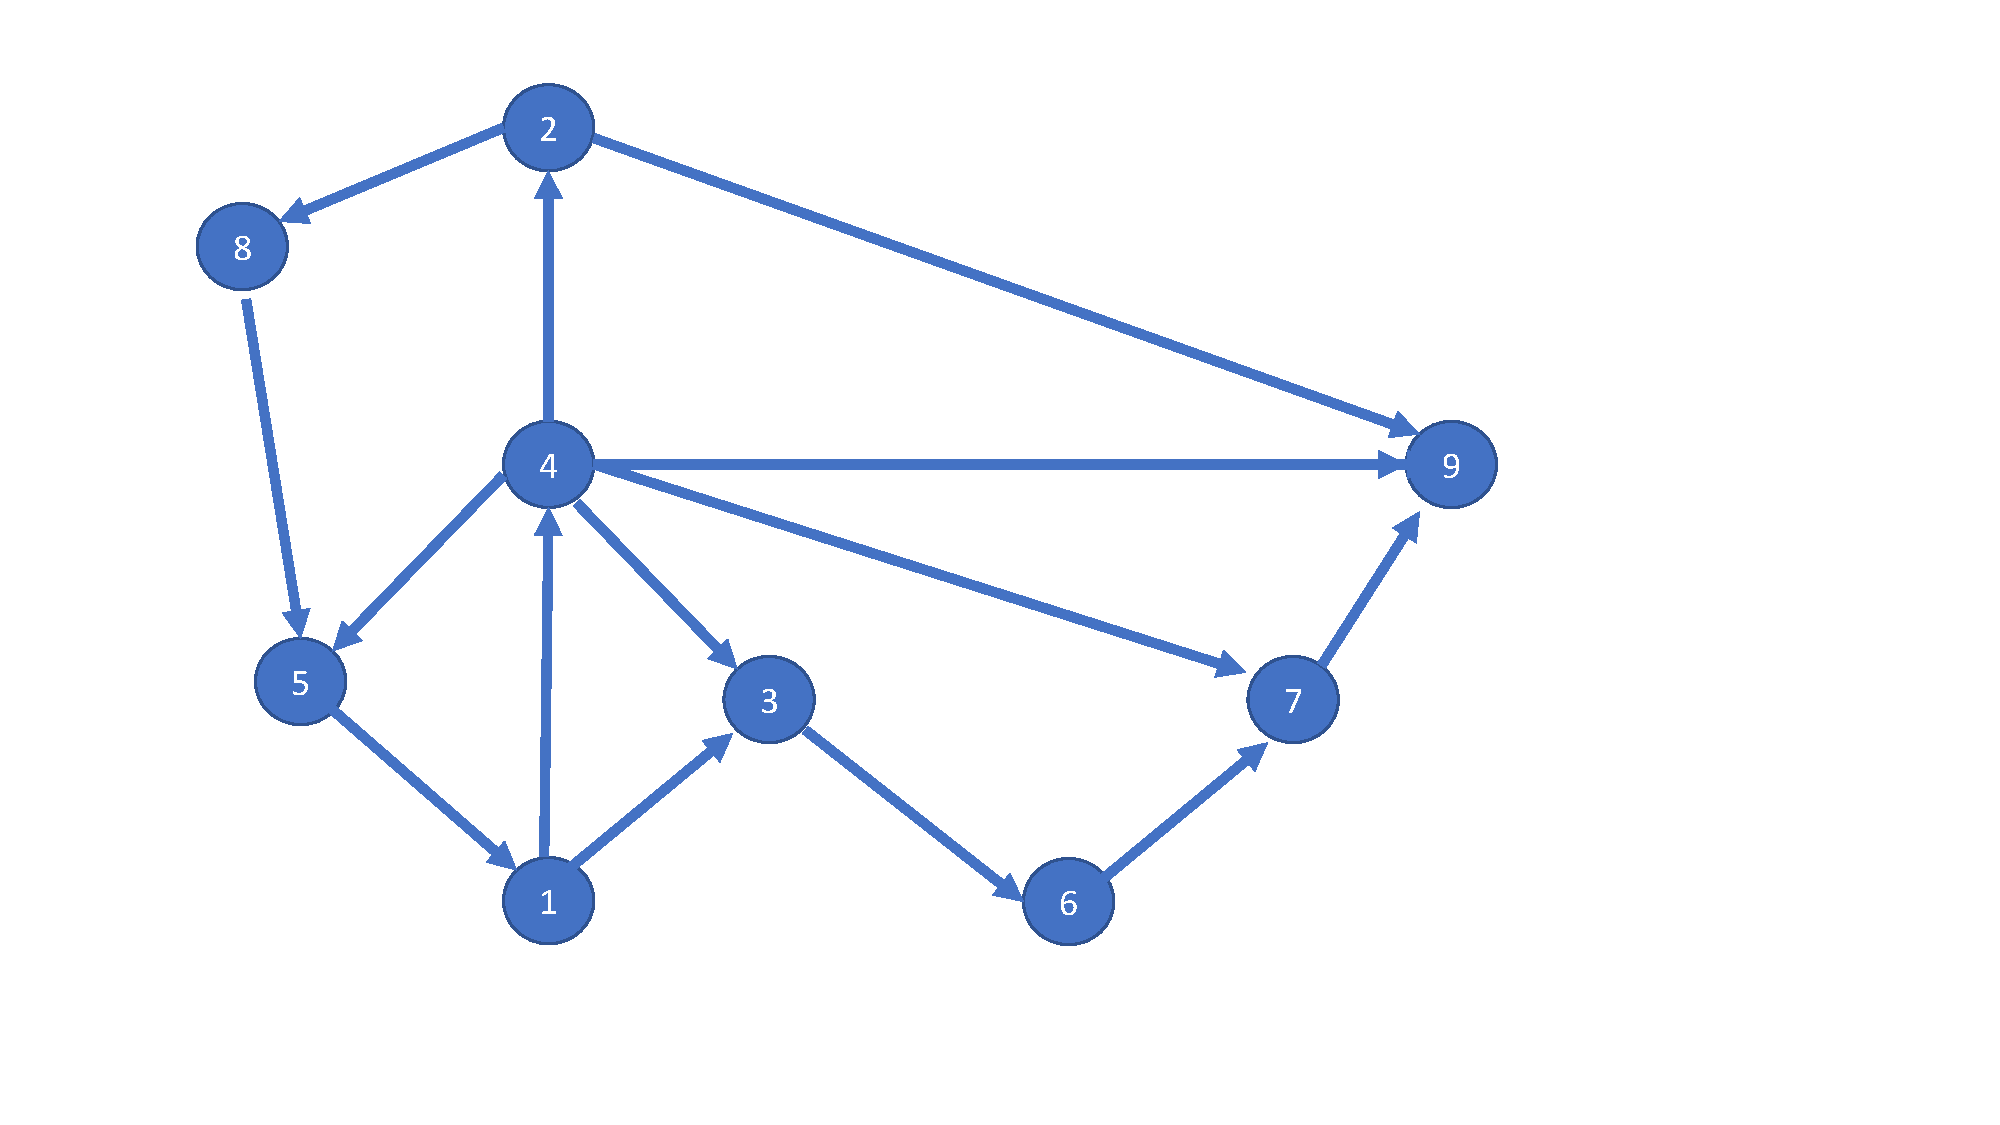
\includegraphics{DFS.pdf}}}
		\caption{The input graph for Question 4.}
		\label{fig:DFS}
	\end{figure}
	
	\end{question} 
	
	%\begin{question}[15 points]\\  
	
%	You are running Dijkstra's algorithm on a directed graph $G =(V,E)$. While Dijkstra's algorithm is executing you realize that a new edge $(u,v)$ should be added to the graph. Vertex $u$ has already been removed from the priority queue, PQ, maintained by Dijkstra's algorithm. Vertex $v$ has no other incoming edge than from $u$. In PQ,   you still see a vertex $w$ with $cost(u,w) <  cost(u,v)$. I now claim that it is ok to add the
%	$(u,v)$ without creating errors. We only have to put it  into the PQ. Which priority value should $v$ have in the PQ? Why would this work?
	
%	\end{question} 
	\newpage
	\begin{question}[15 points]\\  
Consider the following linear program.
\begin{align*}
 & \text{minimize} & 2x_1+3x_2& \\
 & \text{subject to} & x_1+1.5x_2\leq 10\\
 &                   & x_1-x_2\leq 3\\
 &                   & x_2\leq 3\\
 &                   & x_1, x_2\geq 0.
\end{align*}
\begin{itemize}
    \item Show the feasible region by plotting the constraints on the $(x_1,x_2)$-Cartesian coordinate system.
    \item Using your feasible region, find the optimal solution for this linear program. Is this the only solution? If yes, then explain why. If no, then state how many optimal solutions are there and justify your answer.
\end{itemize}

\end{question} 
\begin{center}
{\bf End of Assignment}
\end{center}

\end{document} 
